\documentclass[a4paper]{jpconf}
\usepackage{graphicx}
\usepackage{textcomp}

\begin{document}
\title{Systematic profiling to monitor and specify the software refactoring process of the LHCb experiment}

\author{Ben Couturier$^{1}$, E. Kiagias$^{2}$ and Stefan B. Lohn$^{1}$}
\address{$^{1}$ CERN, CH-1211 Geneva 23, Switzerland}
\address{$^{2}$ University of Athens, Greece}

\ead{ben.couturier@cern.ch emmanouil.kiagias@cern.ch stefan.lohn@cern.ch}

\begin{abstract}
The LHCb upgrade program implies a significant increase in data processing that will not be matched by additional computing resources. Furthermore, new architectures such as many-core platforms can currently not be fully exploited due to memory and I/O bandwidth limitations. A considerable refactoring effort will therefore be needed to vectorize and parallelize the LHCb software, to minimize hotspots and to reduce the impact of bottlenecks. It is crucial to guide refactoring with a profiling system that gives hints to regions in source-code for possible and necessary re-engineering and which kind of optimization could lead to final success.
\newline
Software optimization is a sophisticated process where all parts, compiler, operating system, external libraries and chosen hardware play a role. Intended improvements can have different effects on different platforms. To obtain precise information of the general performance, to make profiles comparable, reproducible and to verify the progress of performance in the framework, it is crucial to produce profiles more systematically in terms of regular profiling based on representative use cases and to perform regression tests. Once a general execution, monitoring and analysis platform is available, software metrics can be derived from the collected profiling results to trace changes in performance back and to create summary reports on a regular basis with an alert system if modifications led to significant performance degradations.
\end{abstract}

\section{Introduction}
\label{sec:introduction}

In large-scale software solutions of high energy physics (HEP), performance is critical for efficient result extraction. The LHCb software is constantly evolving. Thus it is important that software is easily maintainable, is flexible for changes and keeps the usability simple for the huge developer community. These considerations may mean that performance has a lesser priority. The many available profiling tools do not change the game, since performance information is not clearly and reliably available to determine the importance of optimization measures. The LHCb performance \& regression (PR) project tries to address this issue for the LHCb experiment.

During its development phase, the LHCb software was constantly optimized; the profiling was however the responsibility of each developer, with no ``official'' profiling test suite defined and no record of the results. While this approach was effective during the initial framework development phase, there is no record of the evolution of software performance of the baseline. With a refactoring of the code under way, it is therefore now necessary for LHCb to put systematic profiling tests in place, in order to ensure that there is no performance degradation.

This paper gives an overview of LHCb software and the objectives of the LHCb PR project in chapter \ref{sec:lhcb_computing}, the work-flow with some technical aspects in chapter \ref{sec:lhcbpr} and briefly goes into upcoming challenges in chapter \ref{sec:lhcbpr_and_beyond}.

\section{LHCb computing}
\label{sec:lhcb_computing}

\subsection{LHCb software}
\label{sec:lhcb_software}

The LHCb experiment software is based on Gaudi\cite{gaudi}, a C++ framework using generic and object-oriented features of C++ for computing intensive tasks, and python for configuring and structuring modules (algorithms, services, tools). Gaudi provides core services and tools for applications to hide complexity and make future development and changes more transparent for users. It is a large-scale framework and is additionally used by ATLAS, Glast, Harp and other experiments.

Online and Offline applications are built on top of Gaudi. Moore is the implementation of the High-Level Trigger (HLT) to decide whether event data will be stored or not, Brunel is responsible for offline reconstruction, DaVinci is the physics analysis framework, Gauss simulates the particle transport and interaction through several detector modules using Geant4, and Boole performs the digitization.

\subsection{Computing environment}
\label{sec:computing_environment}

The LHCb computing environment consists of computing resources of the Worldwide LHC Computing Grid (WLCG), of Cloud Infrastructure and of the HLT farm located at the experiment. Additional, virtualization is used and just recently volunteer computing has been added using Boinc. Some 100k CPUs are involved in the data processing. 
%35 GB/s of recorded data have to be processed by 1500 computing nodes of the Event Filtering Farm (EFF) of the HLT to be reduced to 70 MB/s \cite{lhcb_hlt_opt}.

\subsection{Integrated Profiling}
\label{sec:integrated_profiling}

Instrumentation is a crucial advantage for profiling source-code of large-scale frameworks. Multiple profiling measures have been implemented in the Gaudi framework using the AuditorService \cite{status_gaudi} which provides an interface for executing code between events or algorithms.

Timing information from the operating system's process information is collected using the TimingAuditor. Likewise information can be collected using the Memory- or MemStatAuditor for changes in the memory footprint. Recent work \cite{intel_auditor} conducted by Mazurov and Couturier has shown how to improve precision in profiling the event-loop by using instrumentation routines of Intel's VTune\texttrademark Amplifier API, which can be added using Gaudi's IntelAuditor. Another strategy is to collect information from the performance monitoring unit (PMU) of modern CPU architectures to collect information about hardware usage such as cache-misses, branch-misprediction and more, as done by Kruse and Kruzelecki \cite{modular_monitoring}. Many profilers and instrumentation routines have been integrated to provide tools for developers to profile their code. Still, profilers have never been used systematically.

\subsection{Systematic Profiling}
\label{sec:integrated_profiling}

Three important aspects are crucial for \textit{systematic profiling}. Profiles must be \textit{comparable}, \textit{reproducible} and \textit{representative} to allow regression analysis and to trace back changes in performance to regions in source-code. This approach is called a \textit{top-down} analysis. Anomalies are detected by comparing the general performance, and in case of a performance drawback responsible algorithms have to be pointed out. Successively the scope can be limited to regions in code, like modules (libraries), algorithms, functions or other entities of source-code locations.

Systematic profiling should be limited to a small number of default use cases and a fixed set of reference data to facilitate finding changes in performance which are crucial for production and to point out source-code regions, that are good candidates for performance optimization. Representative reference data are important to avoid variance due to different types of physics. This way differences in execution behavior between two revisions must originate in related source-code changes. Changing the reference set of physics events could later on be used to evaluate the needs of computing resources for upcoming data-taking periods with differing event information.

Furthermore, profiles must be reproducible in order to compare test configurations of executed test jobs. This affects the \textit{job description}, which is given by version/platform/host information, as well as the \textit{run configuration}, which is providing the setup of a run by an option (configuration) file. As soon as tests are reproducible with representative and reliable results evaluated through multiple runs, tests become comparable for further examinations.

Hence the LHCb PR project has the following requirements.
\begin{enumerate}
 \item Performance information must be centrally collected and become easily accessible. A web application as interface to support brief analysis of collected data could achieve this, while additionally facilitating the propagation of issues.
 \item Profiling is a changing subject with new interesting technologies. A solution must be flexible to include information collected with new profiling tools.
 \item Regular execution is necessary to comply with the objective of a reliable regression analysis. An automated chain of triggering, setup, execution and data collection simplifies repetitions of a kind of job and regular execution for changing job configurations.
\end{enumerate}

\begin{figure}
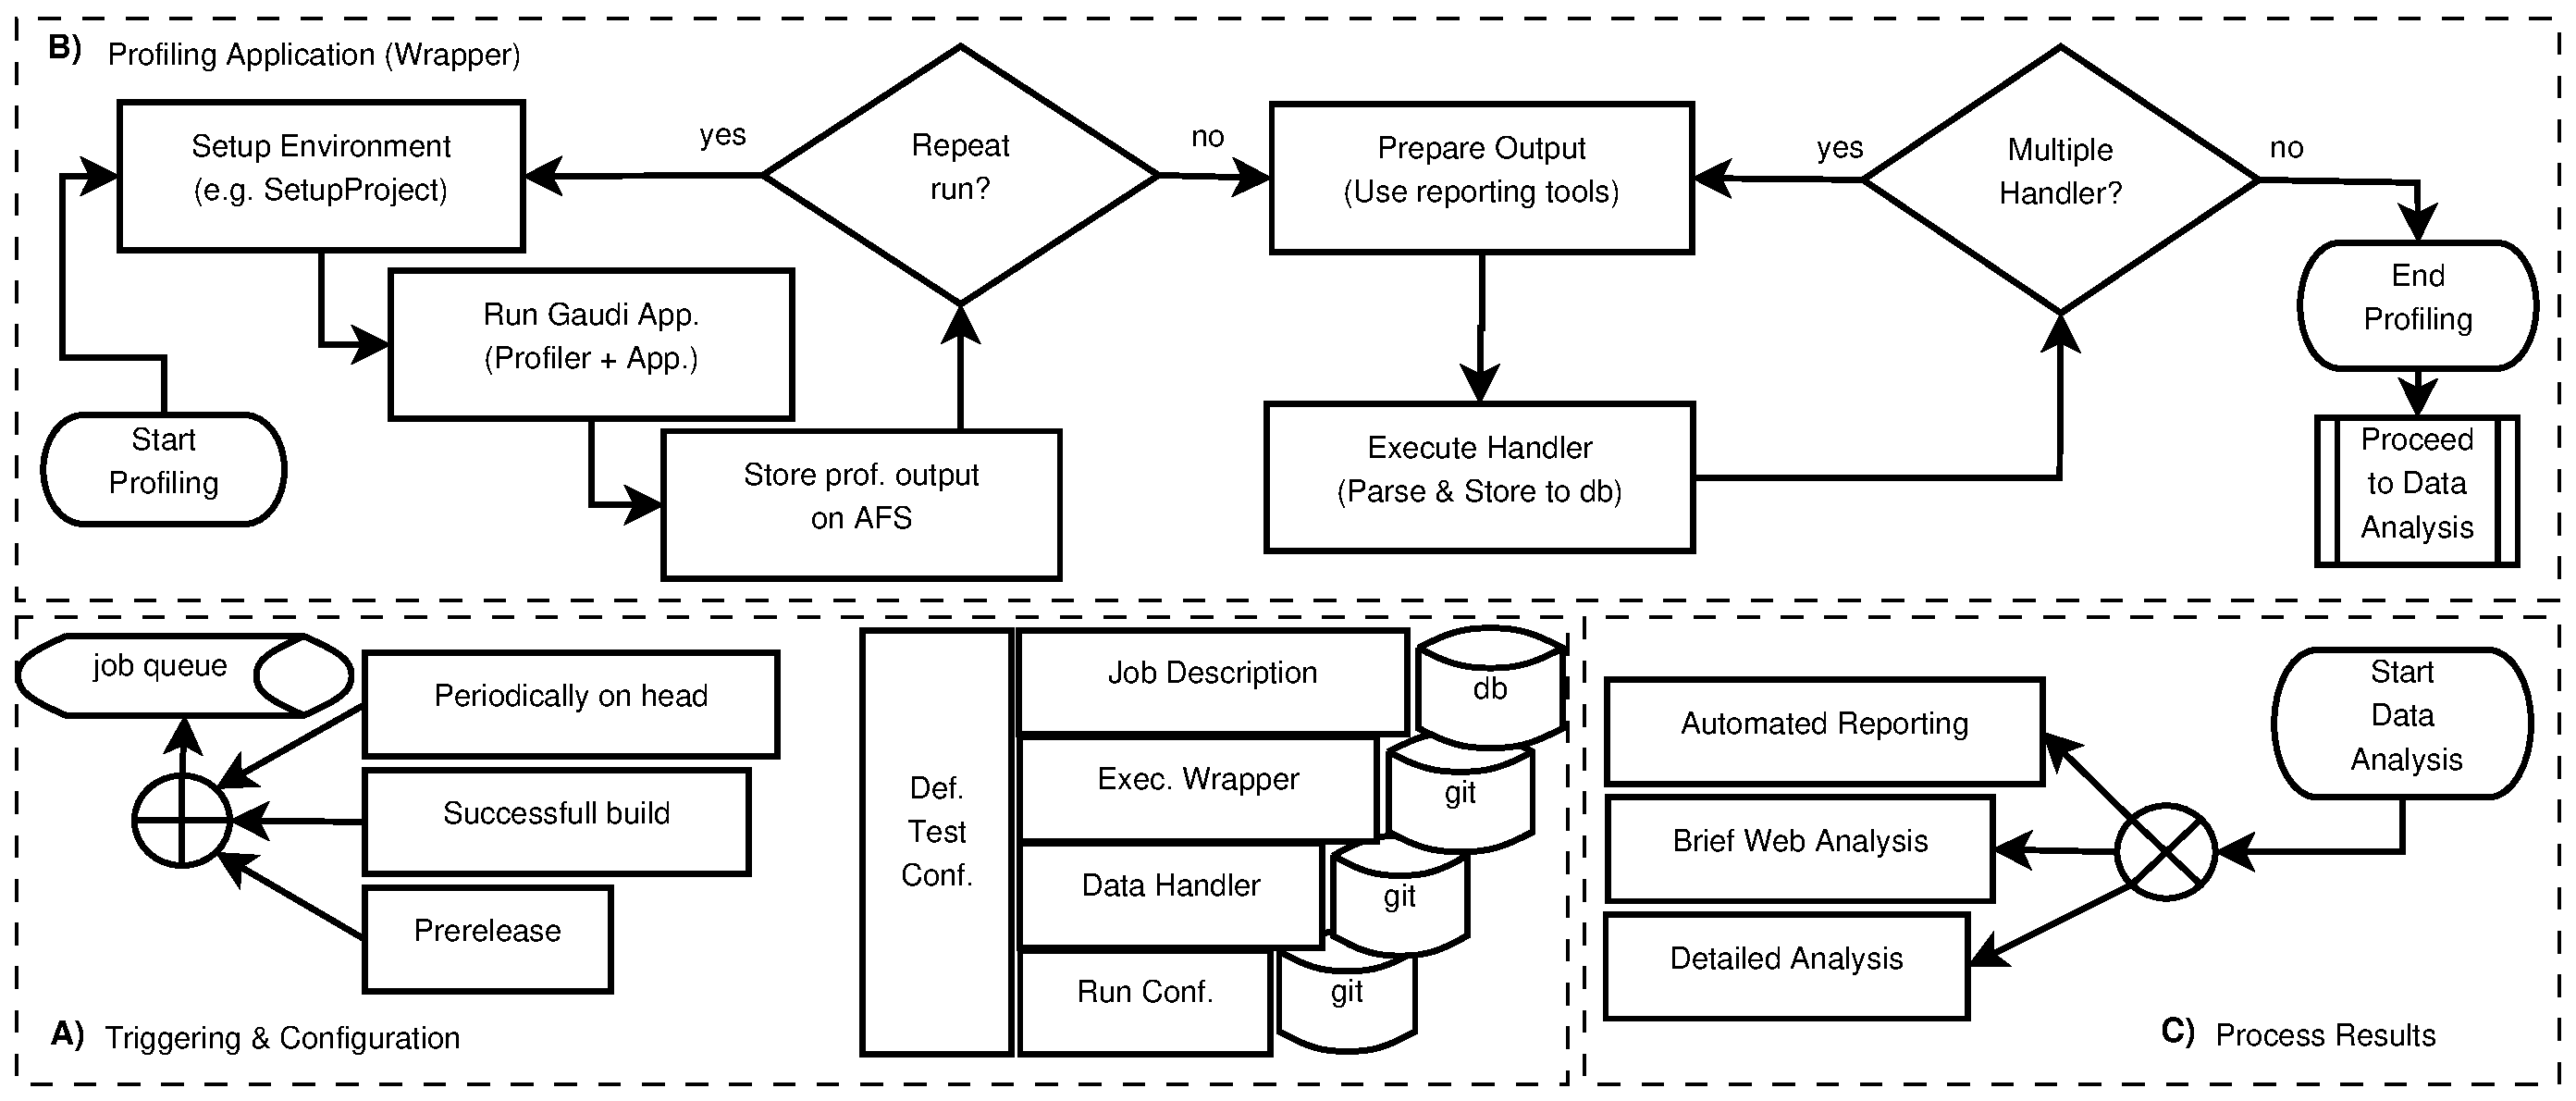
\includegraphics[width=\textwidth, height=5.6cm]{figures/profiling_process.eps}
\caption{\small \textit{The work-flow has three main parts. A) the test definition, triggering and job submission. B) the job execution, repetition and data collection using data handlers. C) quick access to profiling results.}}
\label{fig:profiling_process}
\end{figure}

\section{LHCb PR project}
\label{sec:lhcbpr}

\subsection{Work-flow}
\label{sec:workflow}

The LHCb PR project provides support to conduct systematic profiling. To fulfill the objectives and requirements the work-flow can technically be divided into three major parts, as shown in \mbox{figure \ref{fig:profiling_process}}. In (figure 1A), for reproducibility, the job description and run configuration must be referenced to the collected profiling results from a central relational database. The job description and run configuration is characterized by a job description ID provided by the database, while option files are stored in the version controlled PRConfig package. Jenkins \cite{jenkins}, a continuous integration system, is now used to manage the test configuration, to trigger profiling and submit test jobs for a certain automation of profiling and integration into the software life cycle.

Before the profiling run (figure 1B), a wrapper to setup and start the requested configuration is generated and executed. During execution the profile is acquired and stored on a distributed file system (AFS) or locally. Reports are generated from profiles. Afterwards data handlers for parsing reports and collecting results are called. Results are stored in a relational database, while locally generated files are pushed onto storage to make them accessible via the web based analysis application. In the end of the process (figure 1C) profiles can be easily examined and compared using the LHCb PR web analysis interface. Any anomalies in performance, currently only on algorithm level, can be detected. 

\subsection{LHCb PR web interface}
\label{sec:lhcbpr_web_interface}

The core of the LHCb PR framework is a web interface based on \mbox{Django \cite{django}} to analyze profiles. The backbone of Django is using python to speed up development while keeping a certain amount of flexibility due to a variety of auxiliary modules available. Processing intensive tasks can be performed on the server-side while keeping the interface, on client-side, quick and smart.

The front-end can roughly be divided into two main aspects, navigation and visualization. To \textit{navigate} easily through data, results can directly be accessed by their category, where jobs from a specific job description and run configuration belong to the same \textit{category}. A generic selection menu allows to select specific categories, which one wishes to compare. The generic menu is supplemented by a customized part, to specify profiling groups (different profiling information), attributes or filtering options, which can differ for specific visualizations. Performance information are also available on per job level via a job table with jobs grouped by categories. Here, each single job can be selected and examined.

Different analysis types are referring to different \textit{visualization} methods, in which data \textit{attributes}, generic items of performance information, are shown. Attributes can be runtime, resident memory, possibly lost memory or a more complex software metric. The Trend-Analysis, figures out the progress of attributes cross versions or revisions and has been added to observe changes in the general performance during the code evolution. Significant changes become immediately conspicuous, but requires single attributes, e.g. one of many algorithms, to be tracked. The Overview-Analysis is to show several attributes between two versions, platforms or run configurations. Both, Trend and Overview, show entries with their statistical variance. To get more precise information about the distribution of attribute values around their average the Basic-Analysis can be used.

The visualization uses ROOT histograms which are created with pyRoot, the python interface of ROOT, to allow the access from Django modules and Google Charts for visualization performed on the client-side using javascript. The Basic-Analysis is using ROOT histograms with the attributes dimension as x-axis and normalized about the amount of entries on the y-axis, e.g. in \mbox{figure \ref{fig:brunel_basic_libm}}. Visualizations like job tables, trends, treemaps or overviews are implemented using Google Charts, for which data are preprocessed on the server-side.

\subsection{Job distribution and triggering}
\label{sec:job_distribution}

To facilitate \textit{regular profiling} in a series of equal tests to permit statistical evaluations, Jenkins helps managing the job distribution to dedicated test hosts. The test configuration can be prepared by creating generic parametrized jobs on the Jenkins UI. Also preprocessing, e.g. compiling packages with specific compiler flags or using different revisions of packages within a specific application version, can be conducted by a Jenkins job. Furthermore, it organizes the inclusion of hosts and it prevents interferences between multiple jobs running on the same machine by limiting job slots.

A cron-jobs like plugin in Jenkins can be used to schedule the triggering of profiling jobs either by the release or build cycle. This ensures that from triggering to execution and data collection no human intervention is necessary. This simplifies data collection and opens the way to point out reliable and significant changes in the software profile.

\subsection{Data collection}
\label{sec:data_collection}

Data collection is performed by \textit{data handlers}, which are defined for distinct types of profile reports or which can provide additional information like a comment, a profile class or an AFS path per job. There are two different kinds of routines to transfer collected information. One to save numbers or strings to be stored onto the database and a second to upload files which contain further performance information and could later become available from within the interface. The post-processing of a profiling job must prepare parsable reports for the data handlers. The LHCb PR Handler project contains the various data handlers to parse and collect the data.

\begin{figure}[t]
\begin{minipage}[t]{0.34\textwidth}
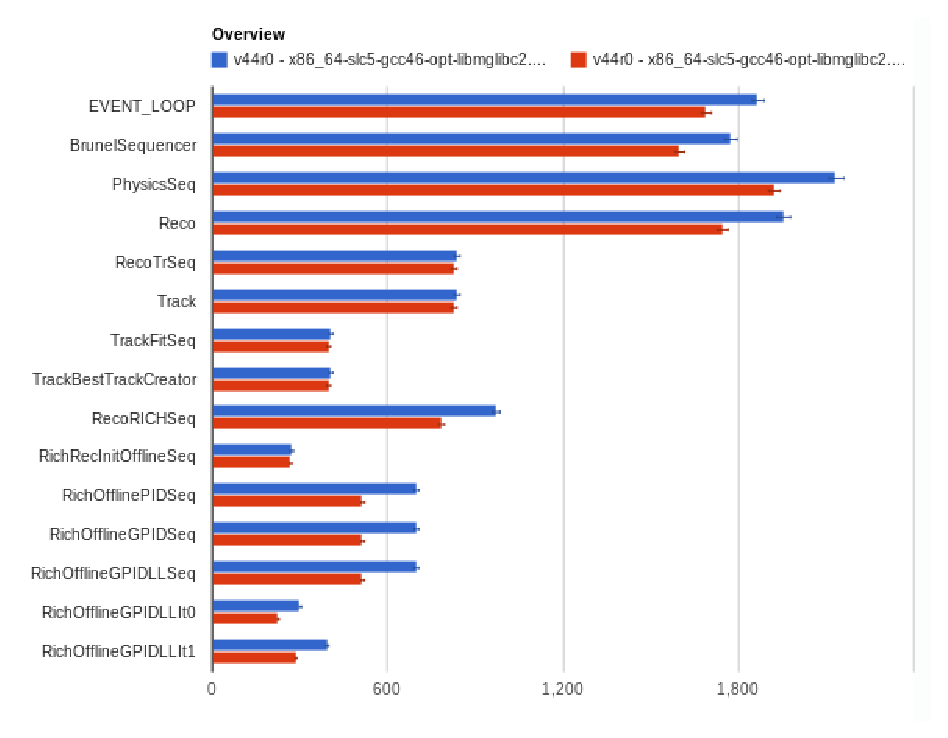
\includegraphics[width=1\textwidth, height=4cm]{figures/brunel_overview_analysis.eps}
\caption{\small \textit{Overview analysis of Brunel to get a fast impression of attributes behavior to others and cross versions, platform or differing configurations (options).}}
\label{fig:brunel_overview}
\end{minipage}\hspace{1pc}
\begin{minipage}[t]{0.29\textwidth}
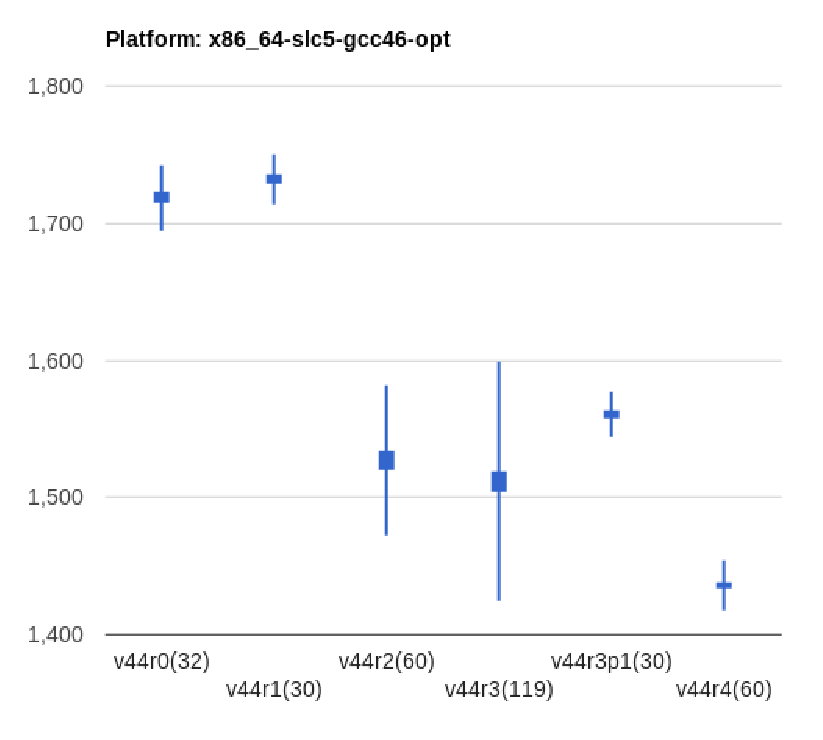
\includegraphics[scale=0.33]{figures/brunel_trend_analysis.eps}
\caption{\small \textit{Trend analysis (runtime [ms] \texttimes\ versions) of Brunel to monitor changes of specific attributes cross versions to observe the general performance.}}
\label{fig:brunel_trend}
\end{minipage}\hspace{1pc}
\begin{minipage}[t]{0.29\textwidth}
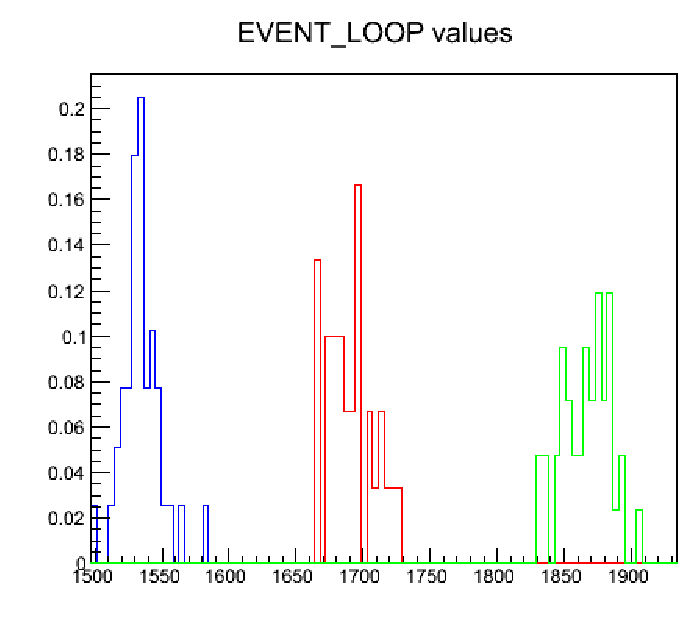
\includegraphics[scale=0.40]{figures/brunel_basic_libm.eps}
\caption{\small \textit{Shows runtime distribution ([ms] per event) using different math libraries. (blue) Intel, (red) elder libm, (green) updated libm of a new glibc version.}}
\label{fig:brunel_basic_libm}
\end{minipage}
\end{figure}

\subsection{Test cases}
\label{sec:test_cases}

Use cases are important to trace performance changes back to the evolving algorithms. \textit{Test cases} are based on \textit{default use cases}, and try to be a best approximation to the production usage. Still, the sophisticated computing environments can influence test runs on a non-predictive non-deterministic way, which hampers conclusions from regression analysis. Currently, the highest priority is to find software related issues, that can be addressed or have to be taken into account for upcoming decisions in resource allocation.

A few default cases for Brunel have been quickly evaluated, defined and are running now on a regular basis after each successful nightly build. LHCb PR has demonstrated its importance already by observing simple timing information obtained by the TimingAuditor. The Overview-Analysis gives a general idea on how single algorithms runtime falls into account, like shown in figure \ref{fig:brunel_overview}. For time consuming algorithms, significant changes become immediately clear by observing the trend information cross versions as shown exemplary in \mbox{figure \ref{fig:brunel_trend}}. After observing performance degradation, further tests can be defined to use more precise profilers, like the IntelAuditor, for more details. One real example shows the changes found in the external math library, as shown in figure \ref{fig:brunel_basic_libm}. Such information needs to be extracted before a release is done.

Unfortunately the HLT framework (Moore) can not simply be reduced to a few common default cases, what makes it more difficult to trace back performance issues using a top-down analysis.

The further complications are:
\begin{enumerate}
 \item The computing environment at the HLT farm is highly sophisticated with processes cloned to save CPU time in initialization, whole node allocation and events coming from the buffer manager.
 \item Single or a few default cases, as required, are not available because of constantly changing trigger configuration keys (TCKs), which define the algorithms involved.
\end{enumerate}

The first problem cannot be addressed since varying runtime caused by the hardware or network hampers performance analysis and the correlation to responsible source-code. The second problem can partially be addressed by splitting one use case into multiple test cases and focusing these cases on specific regions in the source-code. This also simplifies tracing back performance issues to source-code locations and to provide separated development efforts with information.

Finally the Overview-Analysis was adapted to be able to compare different run configurations, to evaluate how separate test cases differ. This way included or excluded algorithms become visible.

\section{LHCb PR and beyond}
\label{sec:lhcbpr_and_beyond}

\subsection{Profiling accuracy}
\label{sec:profiling accuracy}

In the current state, the web-interface does not provide a resolution beyond algorithm level. More detailed information is only accessible via the collected profile information stored on AFS. The resolution of the web-interface is limited for several reasons.
\begin{enumerate}
 \item Systematic profiling with a top-down point of view on performance is to \textit{validate performance}, but not to point to specific lines in code. Hence, LHCb PR currently informs the developer groups about general performance and allows to examine how a specific implementation contributes to the overall performance. Additionally, developers are provided with profiles for detailed analysis for the given default use cases if this is requested. Competing with the variety of good visualization and analysis tools of highly sophisticated profilers would however not be a feasible approach.
 \item Default cases are interesting to \textit{estimate the general performance expectations}, but not to analyze the efficiency of uncommon use cases. Systematic profiling will not completely replace customized profiling by single developers, since uncommon use cases are not covered by the systematic profiling approach.
 \item Regression analysis is gathering, e.g. in the case of thousands of algorithms of a Gaudi application, already big amounts of data with ordinary information. One reason to limit the amount of performance data is, because of the already massive amount of collected data. Statistical evaluations are currently more in focus to provide \textit{reliable and precise information}. Additional limitations are given by the fact that the general performance is characterized by a selection of measurements. Not every measurement will and can be provided.
\end{enumerate}

The higher precision leads already now to further issues, as for instance from the unpredictable side effects of recent hardware features. They can influence runtime on an unreproducible way, e.g. by using frequency scaling or automated over-clocking. On the one hand, these aspects can now precisely be determined, but on the other hand, needs to be neutralized during regular profiling to keep tests reproducible and to detect software performance anomalies.

\subsection{Complementary information}
\label{sec:complementary_information}

Still, it could be reasonable to increase the resolution to function level. A call stack of functions with corresponding runtime would enable us to see if algorithm were using lazy initialization and therefor calling other algorithms first. This is important in particular for Gaudi, which allows a flexible order in which algorithms are executed. E.g. tracking could be triggered by the first algorithm which requests these information. Later on, tracks are only read by the same call. This aspect makes algorithm vary in their runtime. This appears currently as unreasonable change regarding performance of single algorithms.

Furthermore, gathering performance data could be extended by additional information. Correlating specific physics analysis with runtime is frequently performed, but not included into LHCb PR. Likewise different information, like software quality metrics, could be correlated to runtime behavior. Subsequently it would be possible to estimate the impact of design decisions and to find methodologies for new concepts. Open questions could be answered as knowledge base for further developments. Questions like how exactly the call-stack depth causes more cache-misses within a multi-threaded application that is sharing cache among threads, could then be quantified by concrete numbers.

\section{Conclusions}
\label{sec:conclusions}

Using a flexible, extensible and customizable platform to collect and summarize profiling results enables the LHCb collaboration to systematically compare profiles. The LHCb PR project has already demonstrated to be highly valuable. Performance due to changing software and advancing technology is partially examined and issues could be addressed. Since implementing instrumentation is in many aspects already performed and since many profilers can be applied for data collection and since Django and Jenkins is reducing the necessary work to set up a performance monitoring system, the remaining effort is limited to setup a framework for performance and regression analysis, the web application server and to define use cases in collaboration with the developer teams. Still, improvements have to be discussed and put into perspective, but due to the easy adaptivity of the web interface and testing framework, more and more fields for application, like including software metrics, become tangible.

\section*{References}
\bibliographystyle{iopart-num}
\begin{thebibliography}{9}
\bibitem{gaudi} Corti G, Cattaneo M, Charpentier P, Frank M, Koppenburg P, Mato P, Ranjard F, Roiser S, Belyaev I and Barrand G 2006 ``Software for the LHCb experiment'' {\it IEEE Transactions on Nuclear Science} {\bf 53}, nb. 3, P.1323-1328
\bibitem{status_gaudi} Mato P and others 2001 ``Status of the GAUDI event-processing framework'' {\it Computing in high energy and nuclear physics} P.3-7
\bibitem{gaudi_hive} Hegner B, Mato P and Piparo D 2012 ``Evolving LHC data processing frameworks for efficient exploitation of new CPU architectures'' {\it Nuclear Science Symposium and Medical Imaging Conference (NSS/MIC) IEEE} P.2003-2007
\bibitem{lhcb_hlt_opt}Frank M, Gaspar C, Herwijnen E, Jost B, Neufeld N and Schwemmer R 2012 {\it J. Phys.: Conf. Ser.} {\bf 396} 012021
\bibitem{intel_auditor} Mazurov A and Couturier B 2012 {\it J. Phys.: Conf. Ser.} {\bf 396} 052054
\bibitem{modular_monitoring} Kruse D F and Kruzelecki K 2011 {\it J. Phys.: Conf. Ser.} {\bf 331} 042014	
\bibitem{django} ``Django is a high-level Python Web framework'', url: https://www.djangoproject.com/
\bibitem{jenkins} ``Jenkins, An extendable open source continuous integration server'', url: https://www.jenkins-ci.org/
\end{thebibliography}
\end{document}
